\documentclass[12pt]{article}
\usepackage{ctex}
\usepackage{graphicx}
\usepackage{caption}
\usepackage{tabularx}
\usepackage{geometry}
\usepackage{float}  %设置图片浮动位置的宏包
\usepackage{subfigure}  %插入多图时用子图显示的宏包


\geometry{a4paper,scale=0.75}


\title{电力电子技术课程设计}
\author{许文晋}
\begin{document}
\tableofcontents
\pagebreak
\counterwithin{figure}{section}
\counterwithin{equation}{section}

\section{选题背景}
\subsection{自动化技术的发展与意义}
自动化技术发展历史悠久,应用领域广泛。自动化是人们根据科学知识和经验相结合,利用机器实现高效率,高质量,自动化的生产劳动的成果。20世纪70年代,电子技术、传感器技术、控制技术的快速发展推动了自动化技术的发展。特别是计算机的普及使自动化技术有一个质的变化,计算机的发展推动了机器人技术的进步,自动化技术在各个行业的应用越来越广泛。自动化技术的应用提高了劳动效率,提升了产品质量,改善了工作环境。

我国作为一个制造大国,其发展必须是循序渐进的,在这发展的过程中自动化技术的发展是必不可少的。为了更大幅度的提升生产效率,满足日益增长的复杂性生产,自动化技术趋于成熟,这一趋势是无法避免的。

\subsection{YL-335B的自动生产线的基本介绍}
YL-335B的自动生产线由五个基本单元组成,分别是供料单元、加工单元、装配单元、 输送单元和分拣单元,如图1-1是YL-335B的自动生产线布局。我们利用PLC、伺服电机、变频器、组态触摸屏和传感设备,通过PLC控制执行机构,实现生产线工艺流程,利用人机界面进行监视控制,本课题使用的是三菱FX系列PLC,对除分拣站外四个站生产线流程进行设计、调试。对于设备之间的通讯,我们使用三菱FX系列PLC的N:N网络实现工作要求。主要的对输送站为主站,其他单元为从站,互相之间进行响应来实现生产线工艺流程。YL-335B外观如图1-1所示。
\begin{figure}[htbp]
    \centering
    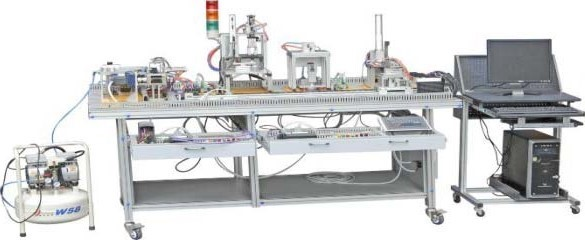
\includegraphics[scale=0.8]{fig/1-1.jpg}
    \caption{YL-335B外观示意图}
\end{figure} 

\section{装配单元结构}
\subsection{管形料仓}
管形料仓用来存储装配用的金属、黑色和白色小圆柱零件。它由塑料圆管和中空底座构成。塑料圆管顶端放置加强金属环,以防止破损。工件竖直放入料仓的空心圆管内,由于二者之间有一定的间隙,使其能在重力作用下自由下落。 

为了能对料仓供料不足和缺料时报警,在塑料圆管底部和底座处分别安装了2个漫反射光电传感器(E3Z-L型),并在料仓塑料圆柱上纵向铣槽,以使光电传感器的红外光斑能可靠照射到被检测的物料上。如图 2-1 所示。光电传感器的灵敏度调整应以能检测到黑色物料为准则。
\begin{figure}[htbp]
    \centering
    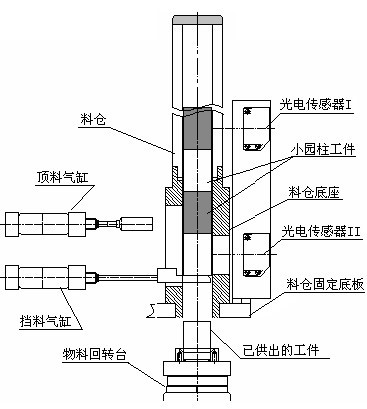
\includegraphics[scale=0.8]{fig/2-1.jpg}
    \caption{落料机构示意图}
\end{figure} 

\subsection{落料机构}
图 2-1 给出了落料机构剖视图。图中,料仓底座的背面安装了两个直线气缸。上面的气缸称为顶料气缸,下面的气缸称为挡料气缸。系统气源接通后,顶料气缸的初始位置在缩回状态,挡料气缸的初始位置在伸出状态。这样,当从料仓上面放下工件时,工件将被挡料气缸活塞杆终端的挡块阻挡而不能落下。需要进行落料操作时,首先使顶料气缸伸出,把次下层的工件夹紧,然后挡料气缸缩回,工件掉入廻转物料台的料盘中。之后挡料气缸复位伸出,顶料气缸缩回,次下层工件跌落到挡料气缸
终端挡块上,为再一次供料作准备。

\subsection{回转物料台}
该机构由气动摆台和两个料盘组成,气动摆台能驱动料盘旋转 180 度,从而实现把从供料机构落下到料盘的工件移动到装配机械手正下方的功能。见图2-2。图中的光电传感器1和光电传感器2分别用来检测左面和右面料盘是否有零件。两个光电传感器均选用CX-441型。
\begin{figure}[htbp]
    \centering
    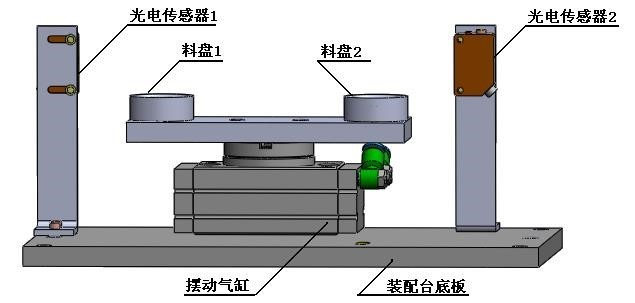
\includegraphics[scale=0.8]{fig/2-2.jpg}
    \caption{回转机构示意图}
\end{figure} 

\subsection{装配机械手}
装配机械手是整个装配单元的核心。当装配机械手正下方的廻转物料台料盘上有小圆柱零件,且装配台侧面的光纤传感器检测到装配台上有待装配工件的情况下,机械手从初始状态开始执行装配操作过程。装配机械手整体外形如图2-3所示。
\begin{figure}[htbp]
    \centering
    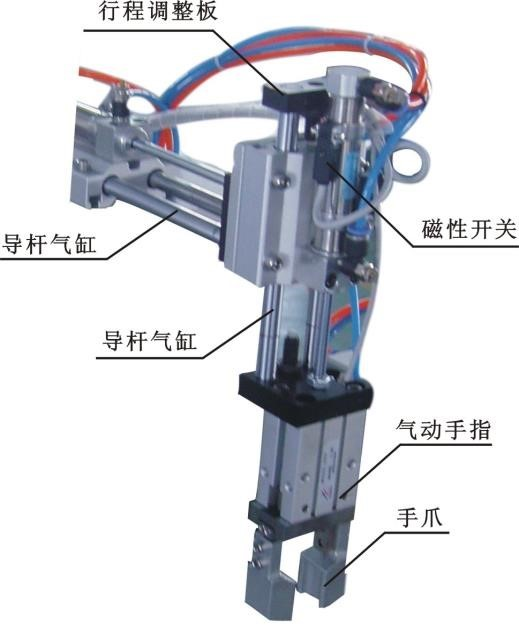
\includegraphics[scale=0.8]{fig/2-3.jpg}
    \caption{装配机械手的整体外形}
\end{figure} 

装配机械手装置是一个三维运动的机构,它由水平方向移动和竖直方向移动的2个导向气缸和气动手指组成。 装配机械手的运行过程如下:

PLC 驱动与竖直移动气缸相连的电磁换向阀动作,由竖直移动带导杆气缸驱动气动手指向下移动,到位后,气动手指驱动手爪夹紧物料,并将夹紧信号通过磁性开关传送给 PLC,在 PLC 控制下,竖直移动气缸复位,被夹紧的物料随气动手指一并提起,离开当廻转物料台的料盘,提升到最高位后,水平移动气缸在与之对应的换向阀的驱动下,活塞杆伸出,移动到气缸前端位置后,竖直移动气缸再次被驱动下移,移动到最下端位置,气动手指松开,经短暂延时,竖直移动气缸和水平移动气缸缩回,机械手恢复初始状态。 

在整个机械手动作过程中,除气动手指松开到位无传感器检测外,其余动作的到位信号检测均采用与气缸配套的磁性开关,将采集到的信号输入 PLC,由 PLC 输出信号驱动电磁阀换向,使由气缸及气动手指组成的机械手按程序自动运行。 

\subsection{装配台料斗}
输送单元运送来的待装配工件直接放置在该机构的料斗定位孔中,由定位孔与工件之间的较小的间隙配合实现定位,从而完成准确的装配动作和定位精度。如图2-4所示。

为了确定装配台料斗内是否放置了待装配工件,使用了光纤传感器进行检测。料斗的侧面开了一个M6的螺孔,光纤传感器的光纤探头就固定在螺孔内。 
\begin{figure}[htbp]
    \centering
    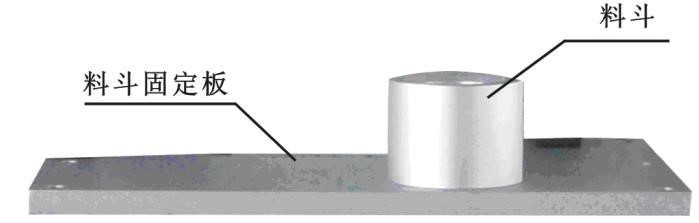
\includegraphics[scale=0.8]{fig/2-4.jpg}
    \caption{装配台料斗}
\end{figure} 
\pagebreak

\section{过程论述}
\subsection{装配单元的结构}
装配单元的功能是完成将该单元料仓内的黑色或白色小圆柱工件嵌入到放置在装配料斗的待装配工件中的装配过程。

装配单元的结构组成包括:管形料仓,供料机构,回转物料台,机械手,待装配工件的定位机构,气动系统及其阀组,信号采集及其自动控制系统,以及用于电器连接的端子排组件,整条生产线状态指示的信号灯和用于其他机构安装的铝型材支架及底板,传感器安装支架等其它附件。其中,机械装配图如图3-1所示:

\begin{figure}[htbp]
    \centering
    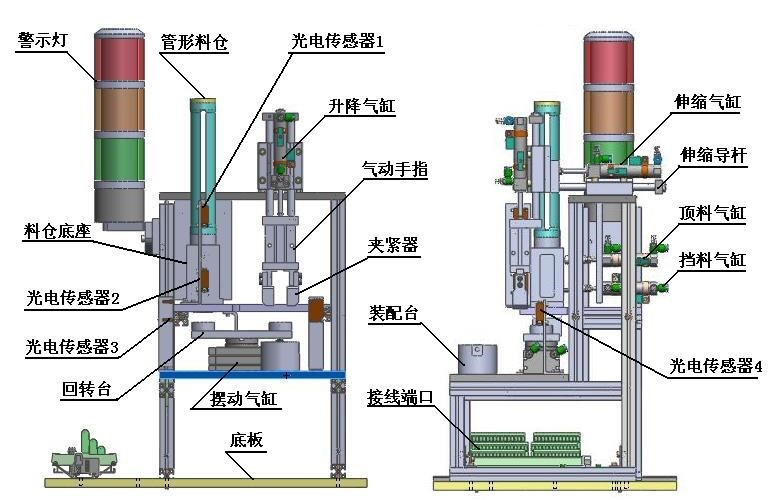
\includegraphics[scale=0.6]{fig/2-6.jpg}
    \caption{装配单元机械装配图}
\end{figure} 

\subsection{装配单元的工作过程}
\subsubsection{工作任务}
1、装配单元各气缸的初始位置为:挡料气缸处于伸出状态,顶料气缸处于缩回状态,料仓上已经有足够的小圆柱零件;装配机械手的升降气缸处于提升状态,伸缩气缸处于缩回状态,气爪处于松开状态。 设备上电和气源接通后,若各气缸满足初始位置要求,且料仓上已经有足够的小圆柱零件;工件装配台上没有待装配工件。则“正常工作”指示灯 HL1 常亮,表示设备准备好。否则,该指示灯以 1Hz 频率闪烁。 

2、若设备准备好,按下启动按钮,装配单元启动,“设备运行”指示灯 HL2 常亮。如果回转台上的左料盘内没有小圆柱零件,就执行下料操作;如果左料盘内有零件,而右料盘内没有零件,执行回转台回转操作。

3、如果回转台上的右料盘内有小圆柱零件且装配台上有待装配工件,执行装配机械手抓取小圆柱零件,放入待装配工件中的操作。 

4、完成装配任务后,装配机械手应返回初始位置,等待下一次装配。 

5、若在运行过程中按下停止按钮,则供料机构应立即停止供料,在装配条件满足的情况下,装配单元在完成本次装配后停止工作。

6、在运行中发生“零件不足”报警时,指示灯 HL3 以 1Hz 的频率闪烁,HL1和HL2灯常亮;在运行中发生“零件没有”报警时,指示灯 HL3 以亮 1 秒,灭0.5秒的方式闪烁,HL2熄灭,HL1常亮。 

\subsubsection{PLC系统接线和I/O分配}
装配单元装置侧的接线端口信号端子的分配如图3-2所示:

\begin{figure}[htbp]
    \centering
    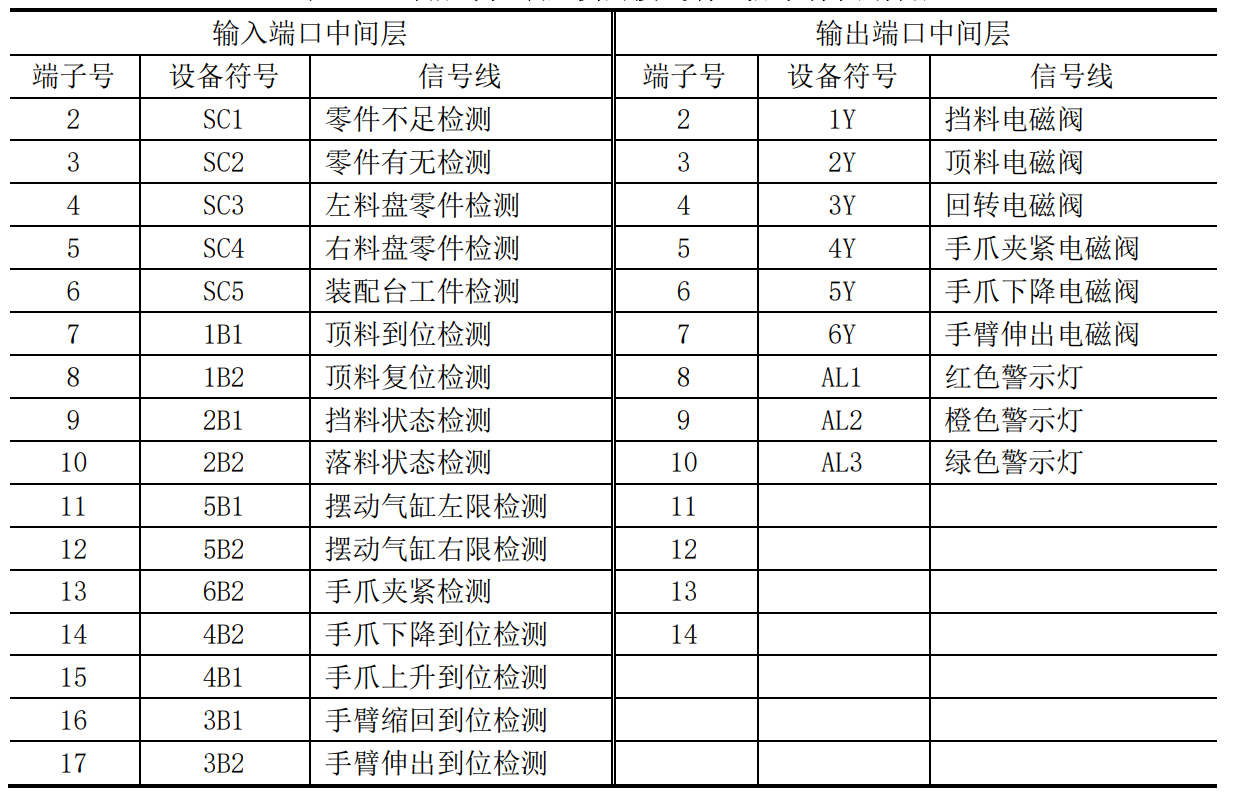
\includegraphics[scale=0.8]{fig/信号端子.png}
    \caption{装配单元装置侧的接线端口信号端子的分配}
\end{figure} 

装配单元的 I/O 点较多,选用三菱 FX3U-48M 主单元,共 24 点输入,24 点继电器输出。PLC 的 I/O 分配如图 3-3 所示。图 3-4 是 PLC 接线原理图。

\begin{figure}[htbp]
    \centering
    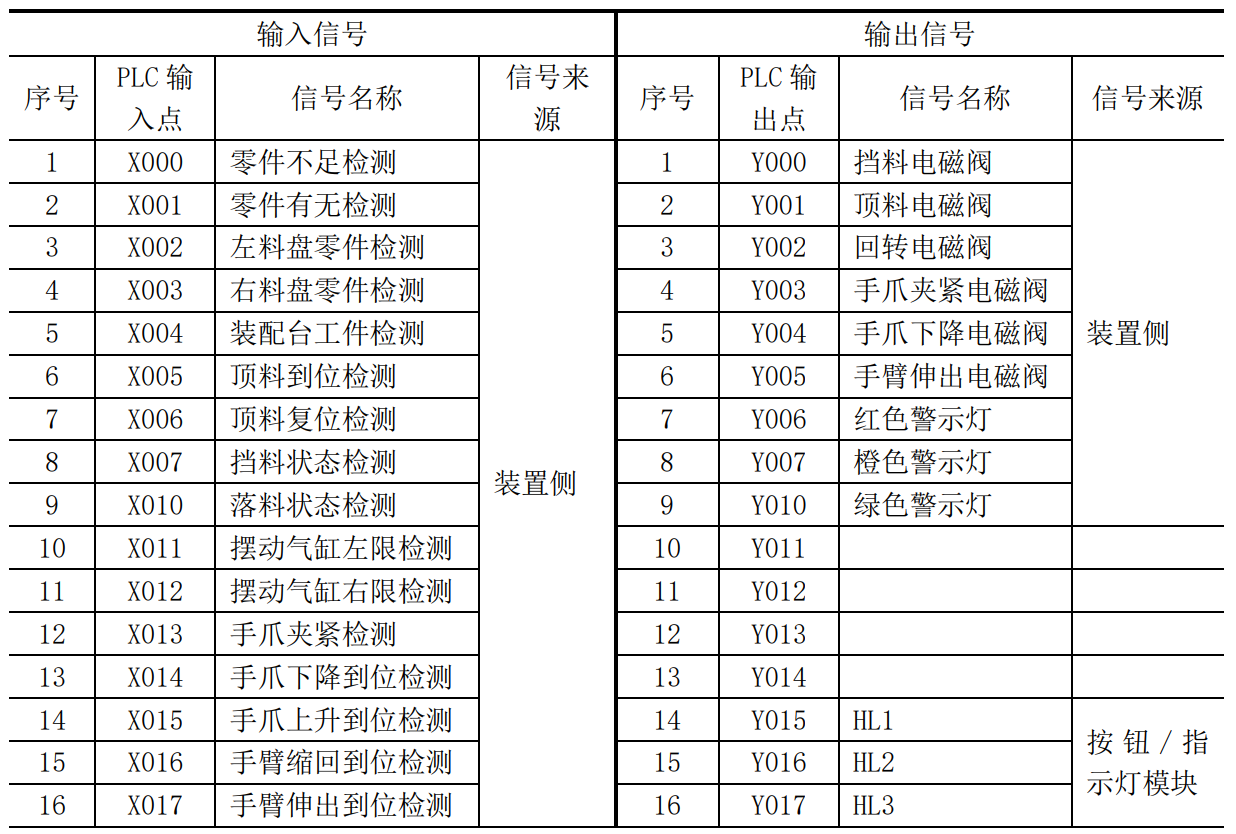
\includegraphics[scale=0.6]{fig/PLCIO.png}
    \caption{装配单元 PLC 的 I/O 信号表}
\end{figure} 

\begin{figure}[htbp]
    \centering
    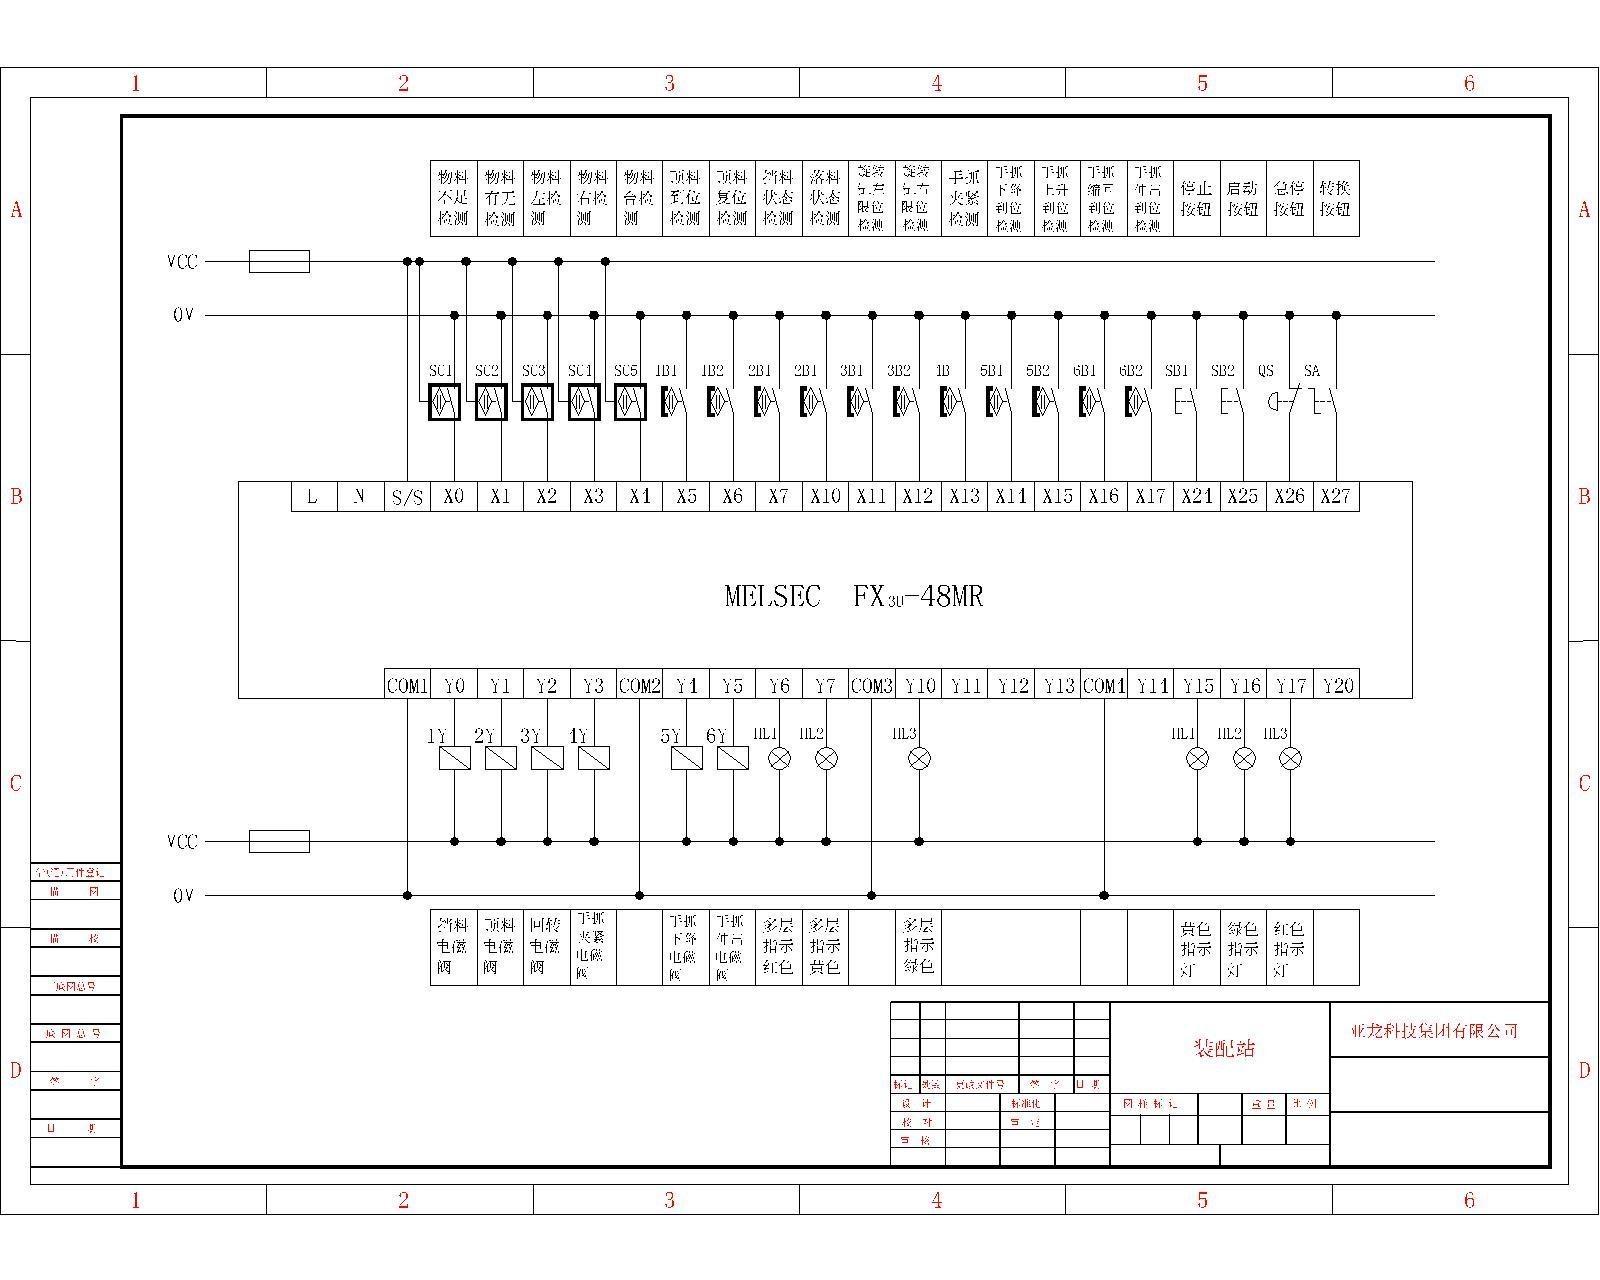
\includegraphics[scale=0.3]{fig/3-4.jpg}
    \caption{装配单元PLC接线原理}
\end{figure} 

\subsubsection{调试与运行}
1、调整气动部分,检查气路是否正确,气压是否合理,气缸的动作速度是否合理。 

2、检查磁性开关的安装位置是否到位,磁性开关工作是否正常。 

3、检查I/O接线是否正确。

4、检查传感器安装是否合理,灵敏度是否合适,保证检测的可靠性。

5、放入工件,运行程序看装配单元动作是否满足任务要求。

装配单元工艺流程图如图3-5:
\begin{figure}[htbp]
    \centering
    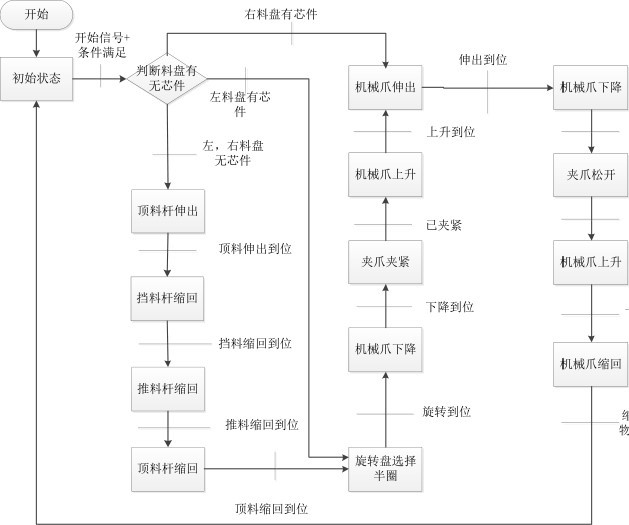
\includegraphics[scale=0.9]{fig/工艺流程.jpg}
    \caption{装配单元工艺流程图}
\end{figure} 

\subsection{装配单元PLC编程}
装配单元梯形图如图3-6,3-7,3-8,3-9所示:
\begin{figure}[htbp]
    \centering
    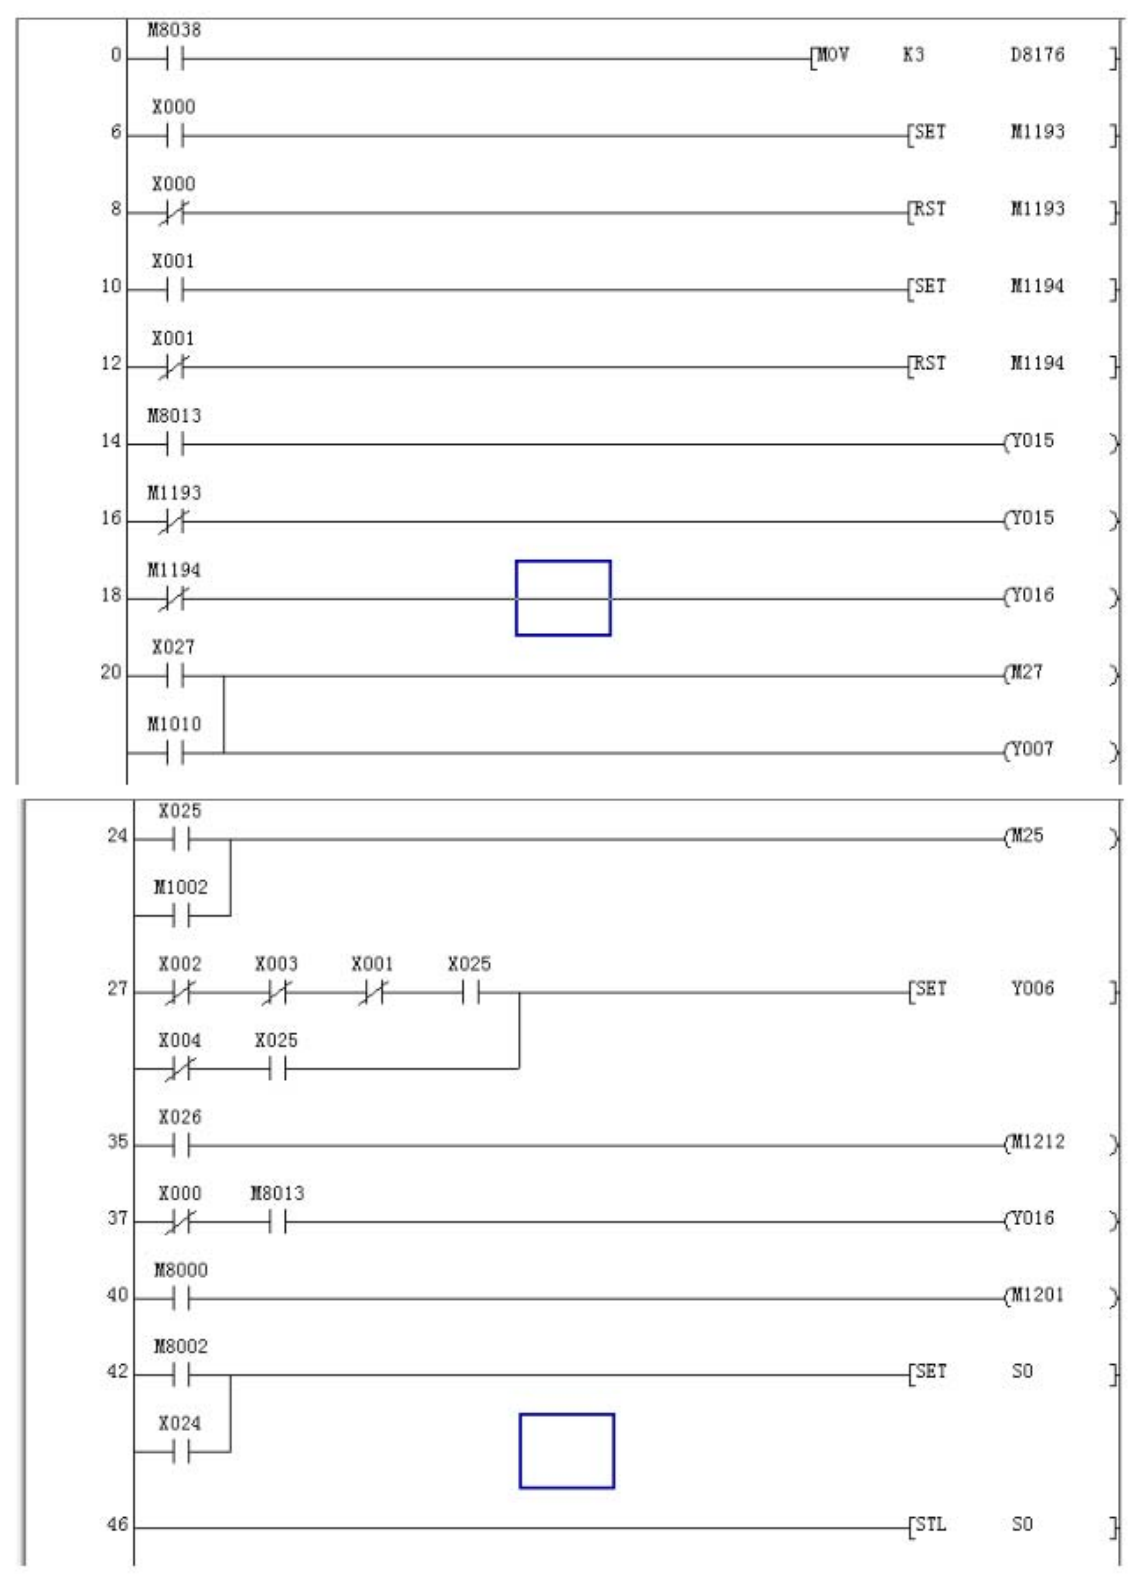
\includegraphics[scale=0.9]{fig/PLC1.png}
    \caption{装配单元梯形图1}
\end{figure} 

\begin{figure}[htbp]
    \centering
    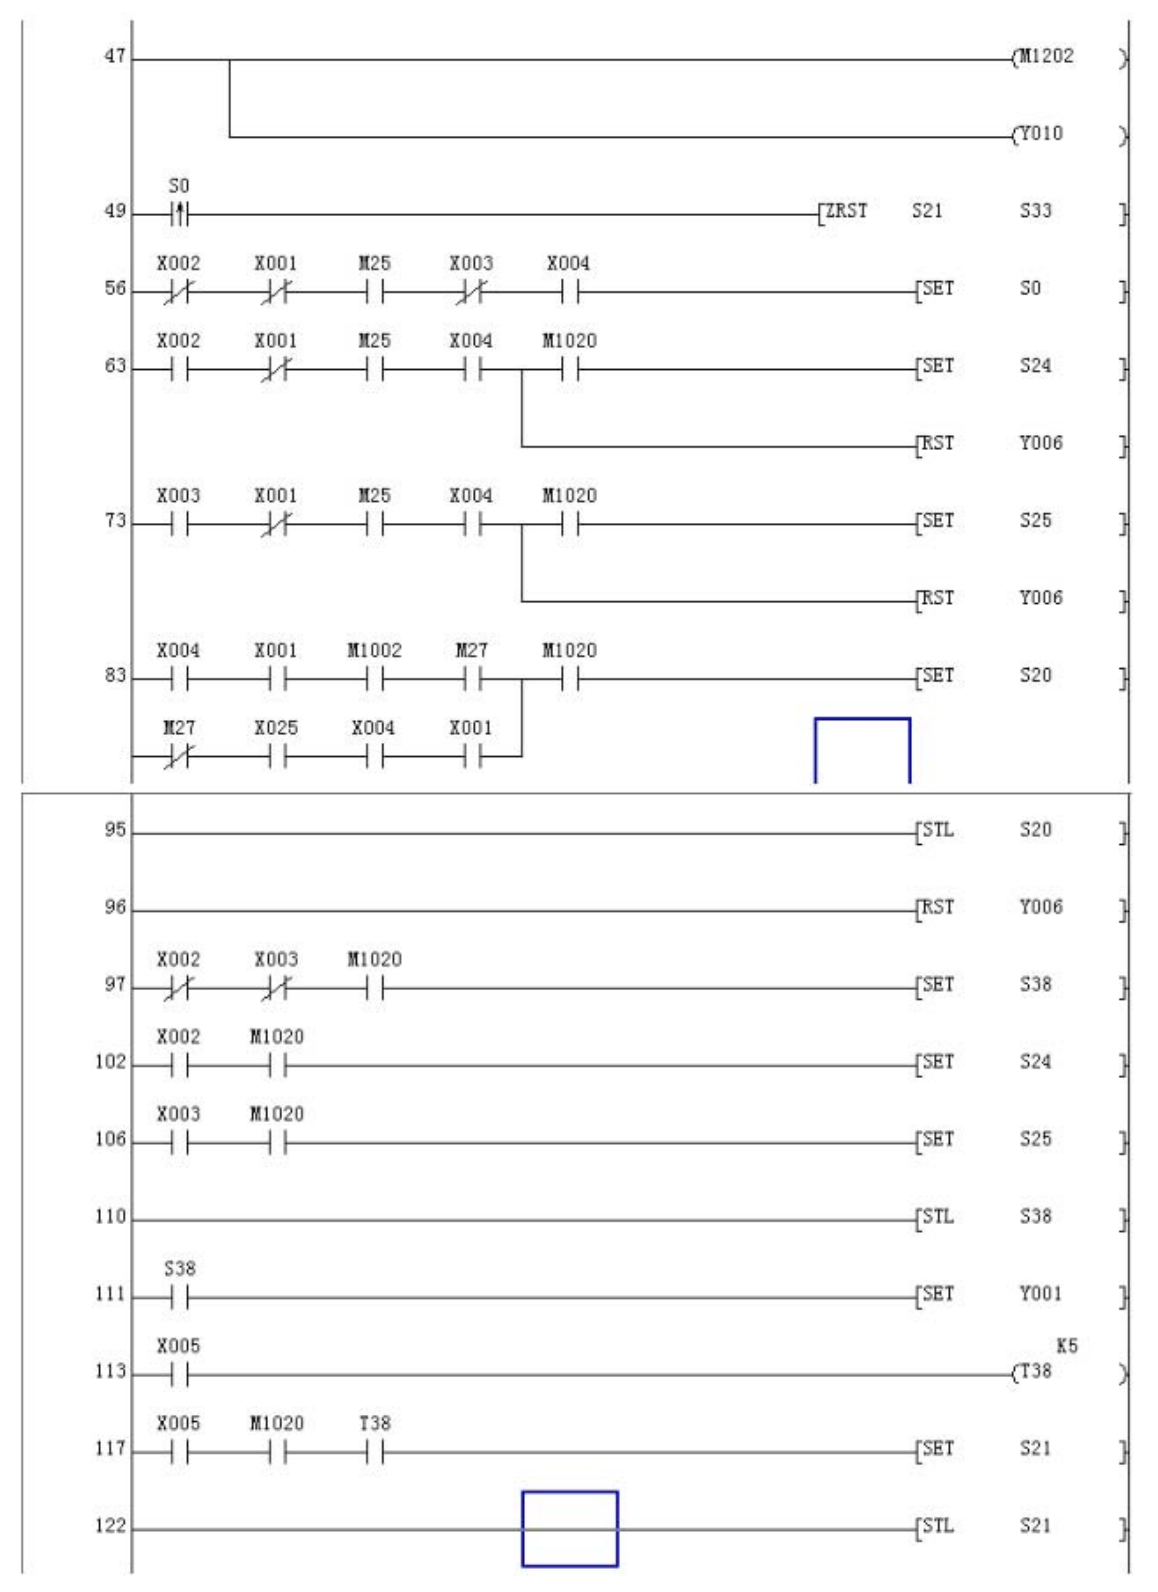
\includegraphics[scale=0.9]{fig/PLC2.png}
    \caption{装配单元梯形图2}
\end{figure} 

\begin{figure}[htbp]
    \centering
    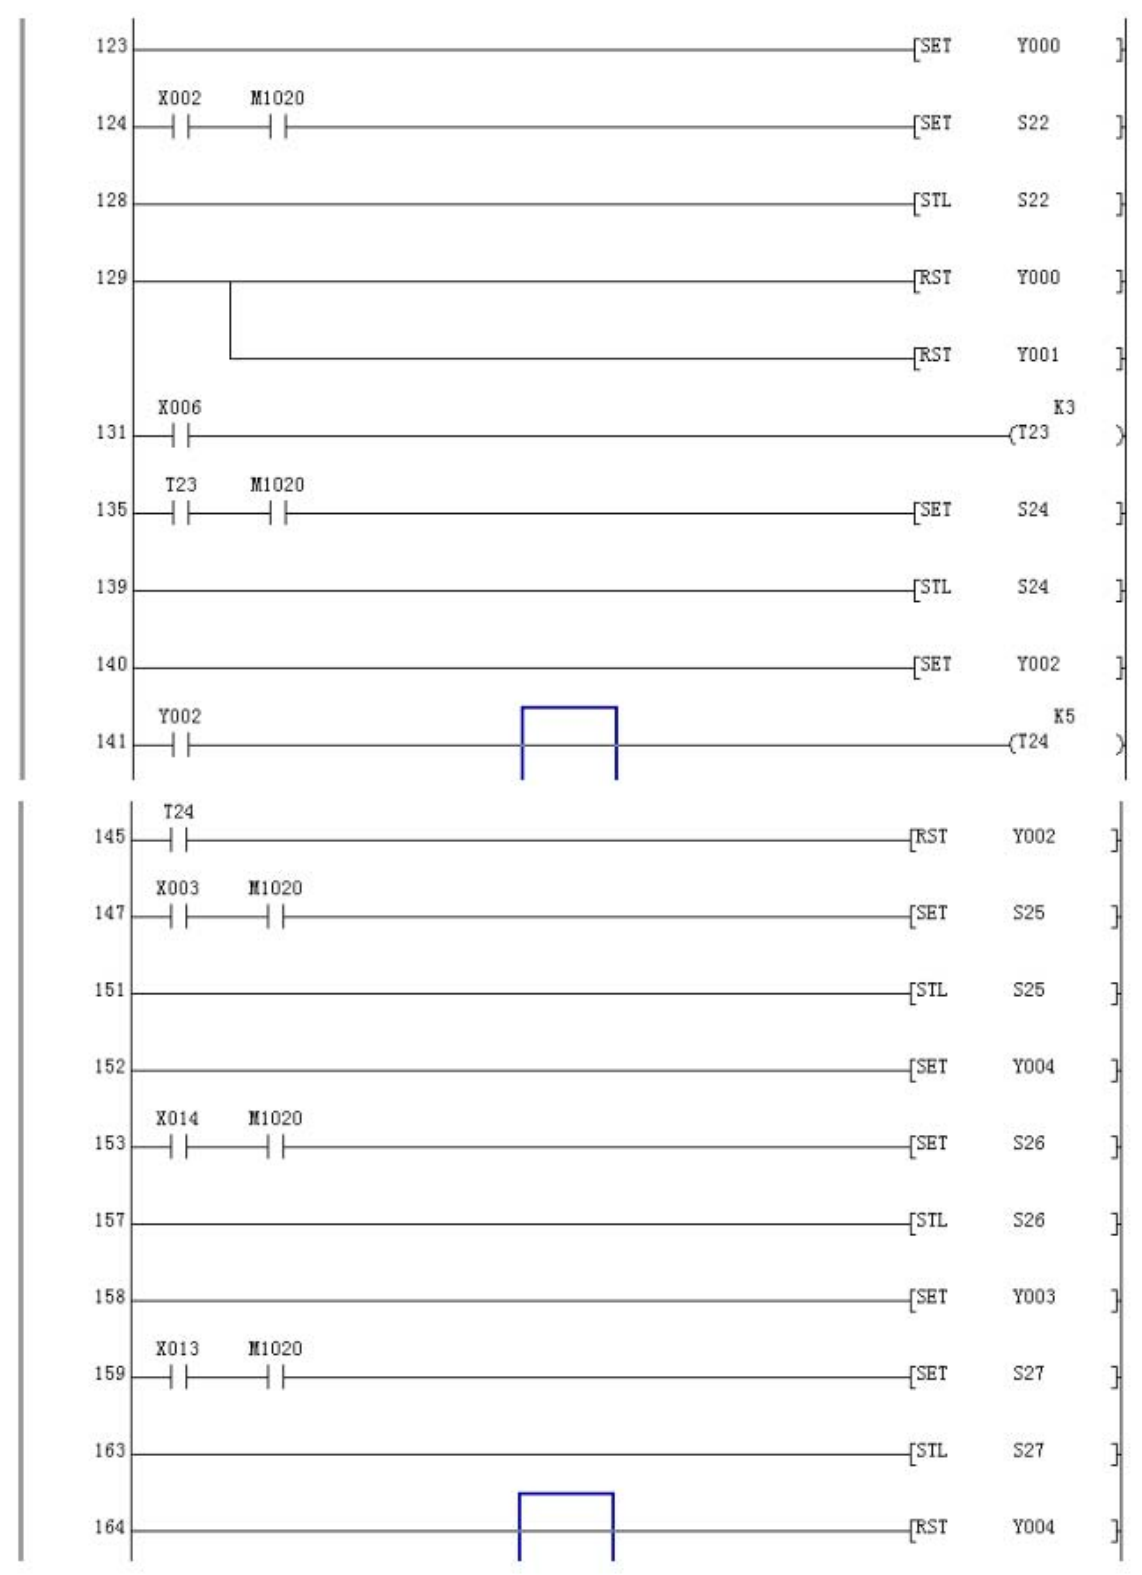
\includegraphics[scale=0.9]{fig/PLC3.png}
    \caption{装配单元梯形图3}
\end{figure} 

\begin{figure}[htbp]
    \centering
    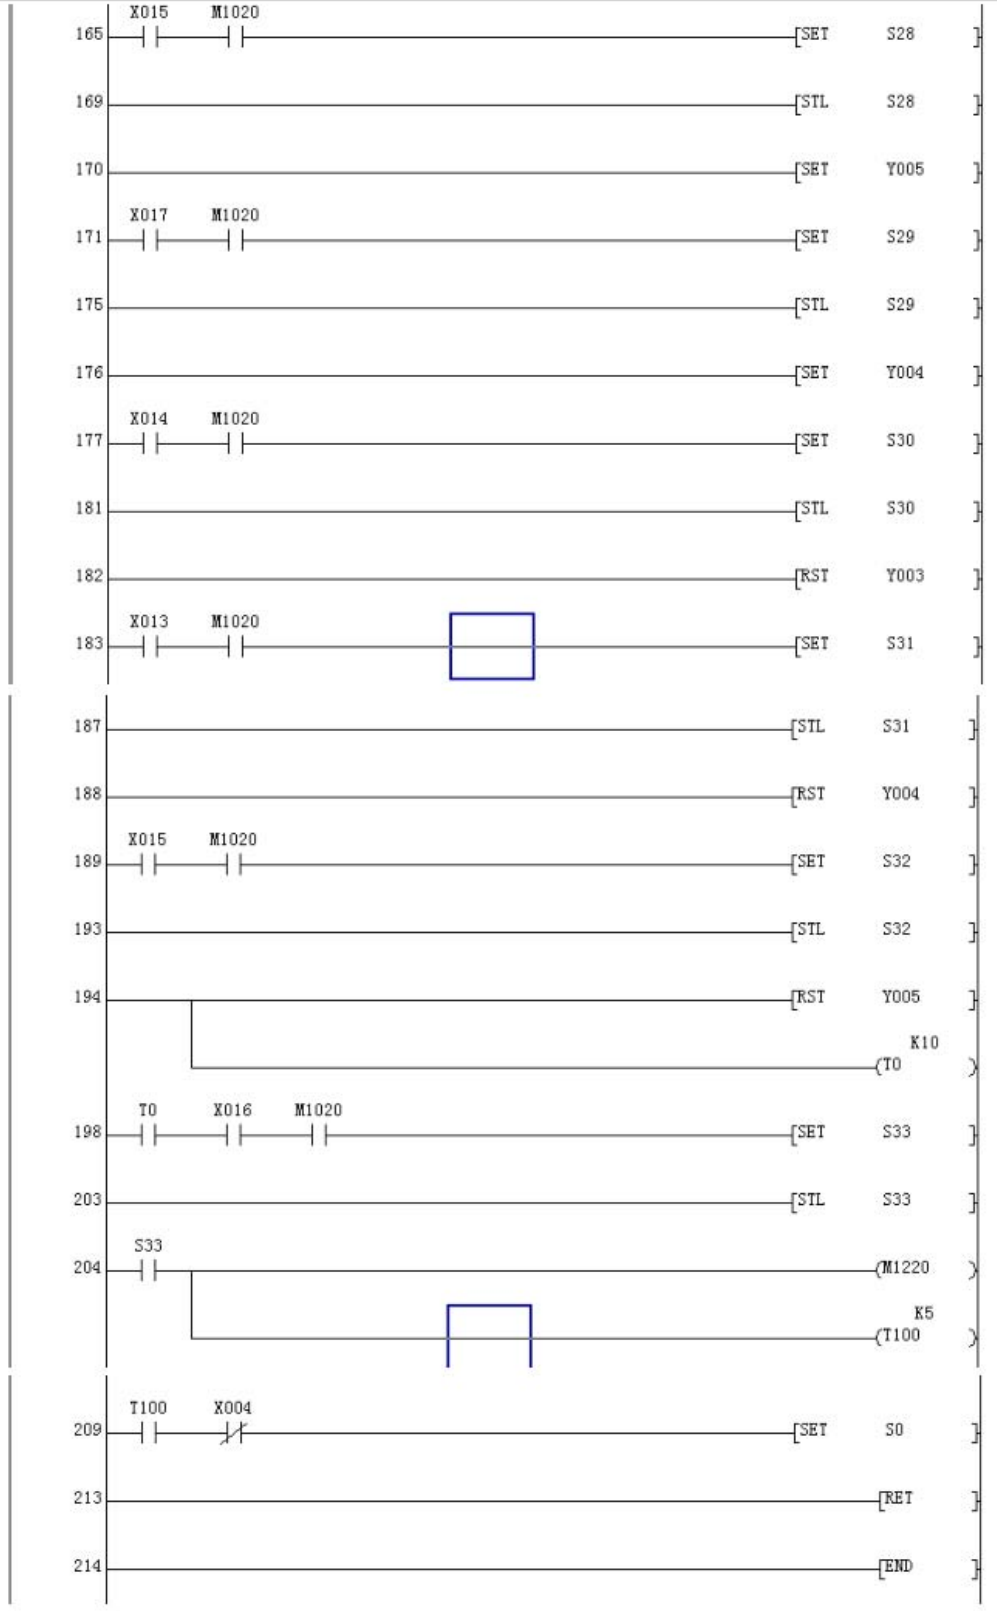
\includegraphics[scale=0.95]{fig/PLC4.png}
    \caption{装配单元梯形图4}
\end{figure} 
\pagebreak

\section{结果分析}
设备上电,气源接通后,各气缸处于原始状态,如果物料台有工件,装配单元可以启动。装配单元启动,若右料盘有工件,夹爪伸出夹取芯件,夹爪缩回,水平气缸伸出,将芯件放至待装配工件中,完成一次装配。完成后各气缸回到原始状态。若左料盘有工件,料盘旋转,夹取完成一次装配。完成后各气缸回到原始状态。左右料盘均无物料进行下料,顶料杆伸出顶住芯件,挡料杆缩回,完成一次下料。旋转物料盘,夹取芯件放至工件台工件中。完成一次装配。完成后各气缸回到原始状态。结果如图4-1所示:

\begin{figure}[h]
	\centering  %图片全局居中
	\subfigbottomskip=2pt %两行子图之间的行间距
	\subfigcapskip=-5pt %设置子图与子标题之间的距离
	\subfigure[fig1]{
		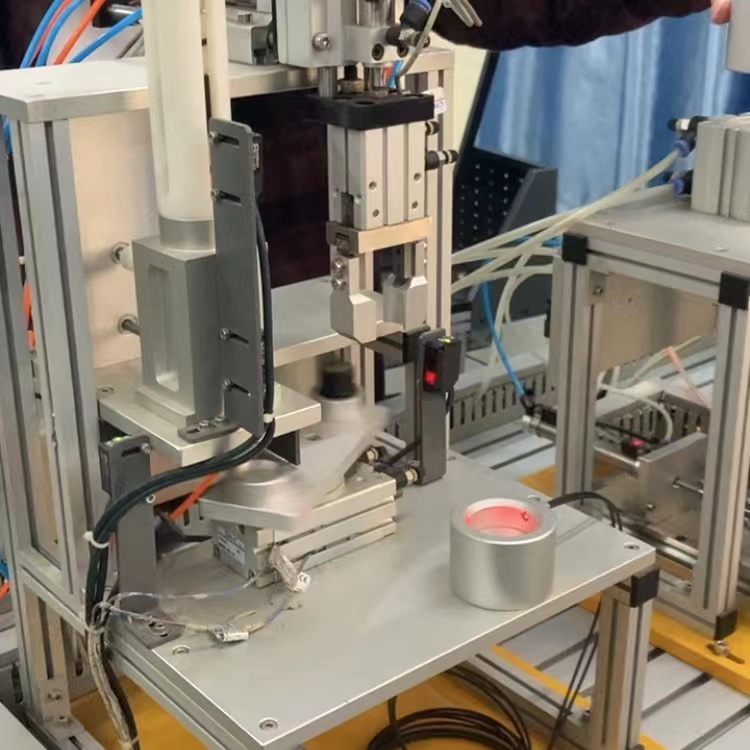
\includegraphics[width=0.3\linewidth]{./fig/r1.jpg}}
	\subfigure[fig2]{
		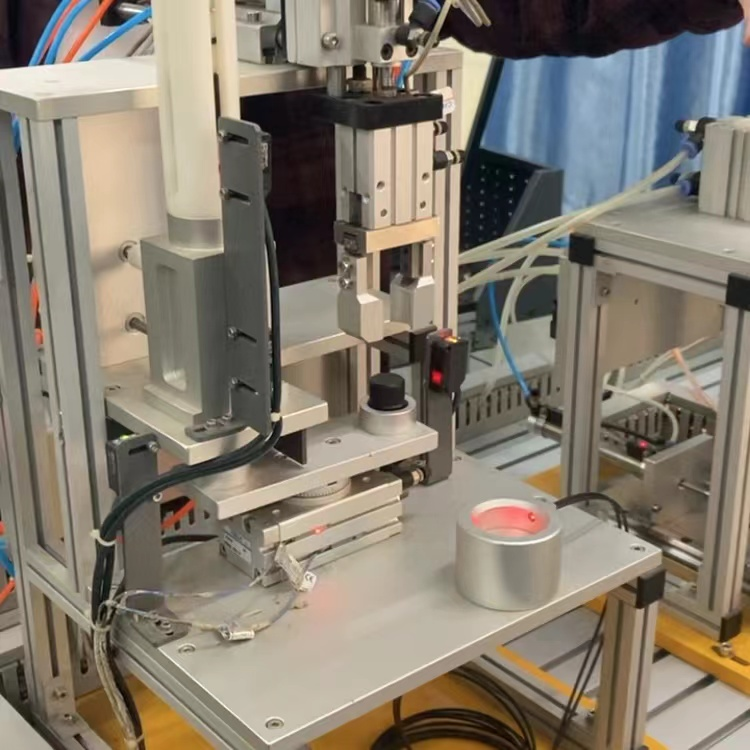
\includegraphics[width=0.3\linewidth]{./fig/r2.jpg}}
	\subfigure[fig3]{
		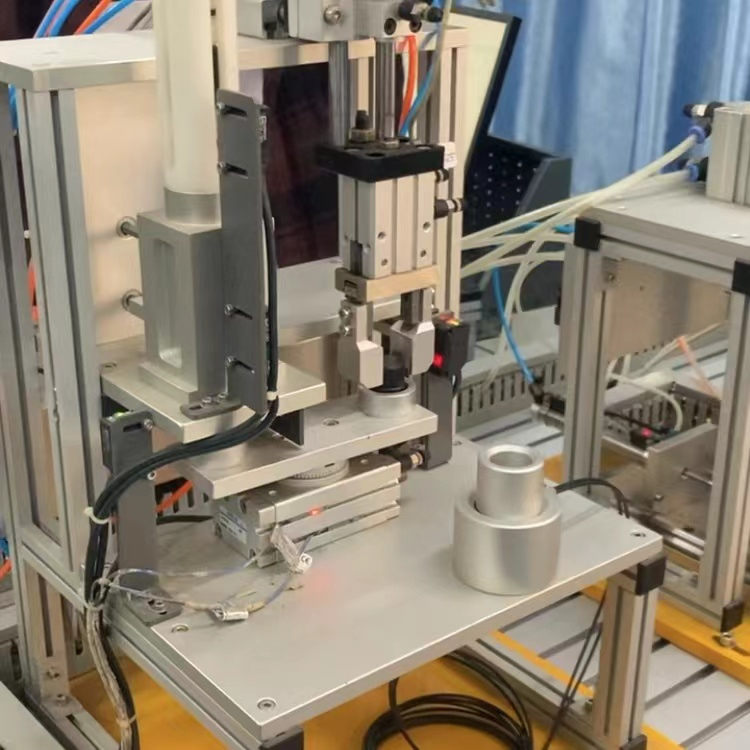
\includegraphics[width=0.3\linewidth]{./fig/r3.jpg}}
    \\
	\subfigure[fig4]{
		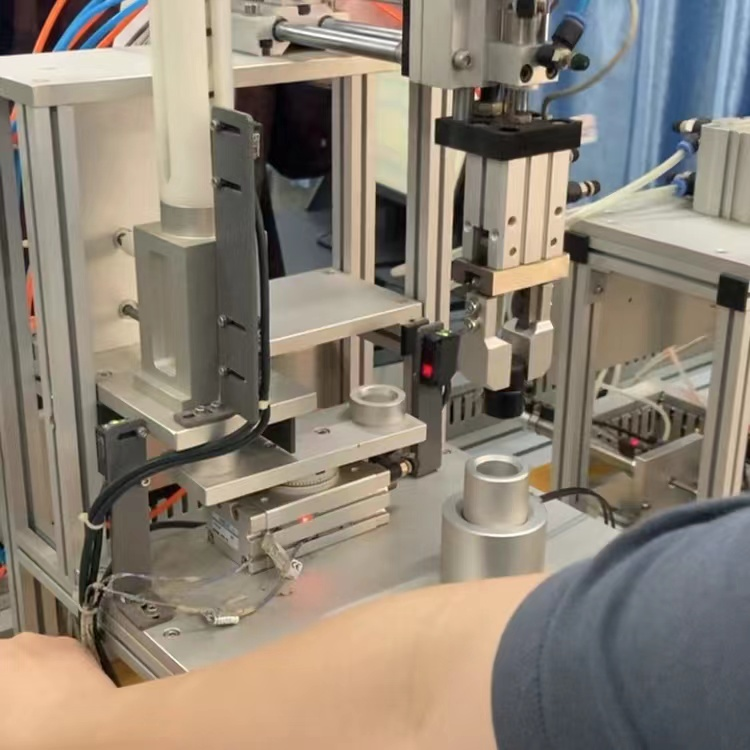
\includegraphics[width=0.3\linewidth]{./fig/r6.jpg}}
    \subfigure[fig5]{
        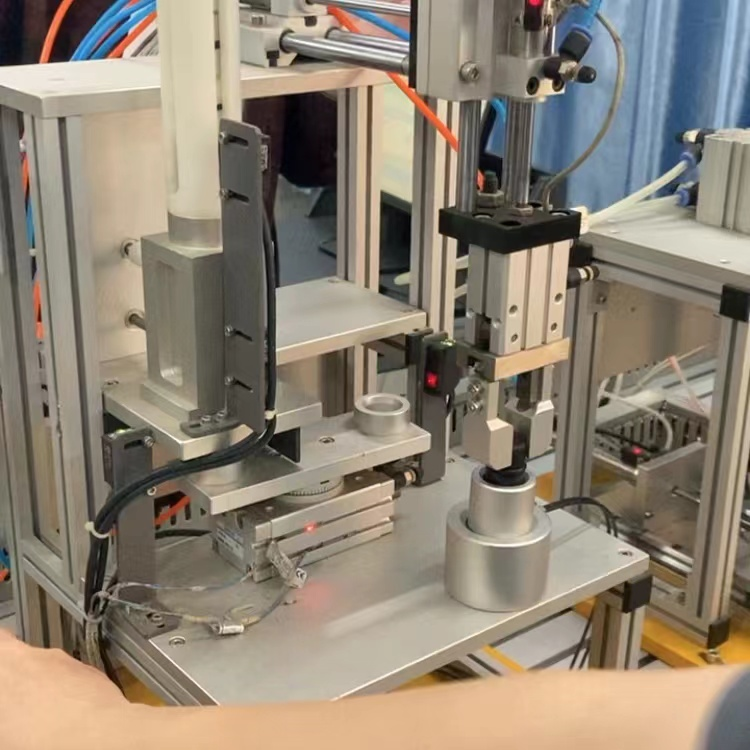
\includegraphics[width=0.3\linewidth]{./fig/r4.jpg}}
    \subfigure[fig6]{
		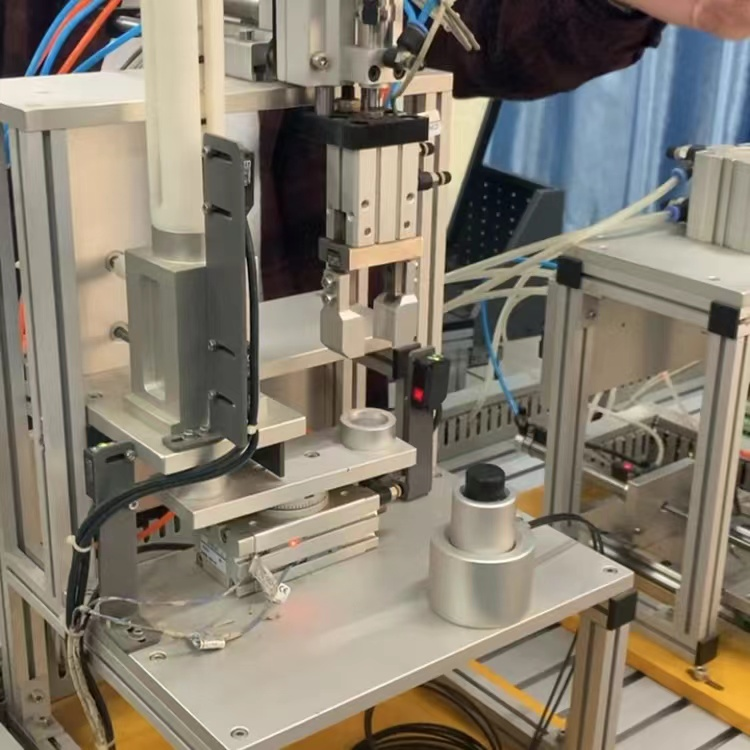
\includegraphics[width=0.3\linewidth]{./fig/r5.jpg}}
	\caption{装配单元运行结果}
\end{figure}

\section{课程设计总结}
从最初阅读任务书时的一窍不通,到最终完成这次课程设计,我从中学到了许多。这次课程设计让我对PLC有了新的认识,与团队的配合也让我学到了团队协作。这次课设让我受益良多。

\end{document}